Mathematicians are often skeptical of proofs relying on extensive computation.
A landmark example is the \emph{four-color theorem}, which states that any planar graph can be colored with at most four colors. 
In 1879, Alfred Kempe published a proof of the four-color theorem, which was discovered to be incorrect 11 years later by Headwood~\cite{Walters2004ItAT,Wilson2002GraphsCA}.\footnote{The main idea of Kempe's proof was salvaged by Headwood to prove the weaker \emph{five-color theorem}, and it is still a building block in the theory of planar colorings~\cite{Walters2004ItAT}.} 
A full proof of the four-color theorem was not found until 1976, when Kenneth Appel and Wolfgang Haken used a computer to check the 1\,834 cases that might contain a counterexample~\cite{appelFourColorProblem1978}.
Their proof was controversial, and indeed, small errors were found in their initial calculations~\cite{Walters2004ItAT,Wilson2002GraphsCA}.
In 2005, Georges Gonthier formalized a full proof of the four-color theorem in the \textsf{Coq} proof assistant~\cite{gonthierFourColourTheorem2008a}, thus laying to rest any lingering doubts about the correctness of the result.
To this day, all proofs known for this theorem require the assistance of computers.

The four-color theorem is far from the end of the story when it comes to computer-assisted mathematics.
An emerging trend is to use SAT solvers (or other automated reasoning tools) to prove mathematical theorems by analyzing finite objects~\cite{avigad2023mathematics}. 
To name a few examples, the Erd\H{o}s Discrepancy Conjecture~\cite{konev2014sat}, Keller's conjecture~\cite{brakensiek2023resolution}, the Packing Chromatic number of the infinite grid~\cite{Subercaseaux_Heule_2023}, and the Pythagorean Triples Problem~\cite{Heule_2016} were all resolved using SAT solvers.
All such SAT-based results follow a common structure: in order to show that a mathematical theorem $\mathcal{T}$ holds, one proves the following:
\begin{enumerate}
  \item (\textbf{Reduction Theorem}) There is a finite object $\mathcal{O}$ such that either (\emph{positive case}) if $\mathcal{O}$ exists then $\mathcal{T}$ holds, or (\emph{negative case}) if $\mathcal{O}$ does not exist then $\mathcal{T}$ holds.\footnote{Note that $\mathcal{T}$ can be a statement concerning infinite objects, as for example in the case of Keller's conjecture~\cite{brakensiek2023resolution}.}
  \item (\textbf{Encoding Theorem}) There is a propositional formula $\varphi_{\mathcal{O}}$ such that either (\emph{positive case}) if $\varphi_{\mathcal{O}}$ is satisfiable then $\mathcal{O}$ exists, or (\emph{negative case}) if $\varphi_{\mathcal{O}}$ is unsatisfiable then $\mathcal{O}$ does not exist.
  \item (\textbf{SAT Result}) In the \emph{positive case}, a SAT solver finds a satisfying assignment for $\varphi_{\mathcal{O}}$, and in the \emph{negative case}, a SAT solver finds that $\varphi_{\mathcal{O}}$ is unsatisfiable.
\end{enumerate}

Unfortunately, the formula $\varphi_{\mathcal{O}}$ concerning the existence of $\mathcal{O}$ is often too large or computationally hard to be solved directly, so a fourth step is added to the above method: a \textbf{Re-encoding Theorem} showing that $\varphi_{\mathcal{O}}$ is equisatisfiable with a simpler formula $\phi_{\mathcal{O}}$.
All the examples we mentioned above add this step, and so will we.

One of the benefits of using a SAT solver for mathematical proofs is that in the \emph{positive case}, it is usually possible to construct the desired object $\mathcal{O}$ from a satisfying assignment to $\phi_{\mathcal{O}}$, and then by exhibiting $\mathcal{O}$, the correctness of theorem $\mathcal{T}$ can be easily verified by humans.
The \emph{negative case}, however, is much harder to trust, as the unsatisfiability proofs emitted by SAT solvers are usually too large for human verification, and depend crucially on the correctness of the encoding.\footnote{In the positive case, the correctness of the encoding is not even required, as an incorrect encoding might still lead to obtaining a concrete object $\mathcal{O}$ that satisfies the desired properties, proving the intended theorem regardless.}
% \todo[inline]{CC: I don't like how this paragraph is structured. The negative case isn't inherently \emph{harder}. Instead, the method of verifying the overall result is different: rather than constructing an actual object we can see or compute on, we have to rely on a non-existence result. Thus, the reduction must be correct, as errors can't be caught the same way they can be in a physical construction.\\ BS: I disagree; the NP vs coNP asymmetry is exactly about how easy it is to convince a verifier of existence vs. non-existence results.}
For example, the resolution of the Boolean Pythagorean triples problem required an unsatisfiability proof of 200 terabytes, the largest known to date~\cite{Heule_2016,lambTwohundredterabyteMathsProof2016}.
This raises a fundamental question for computational mathematics:
\begin{center}
  \emph{How can we trust the correctness of a theorem $\mathcal{T}$ that relies on a very long unsatisfiability proof?}
\end{center}
\begin{figure}[ht]
    \centering
    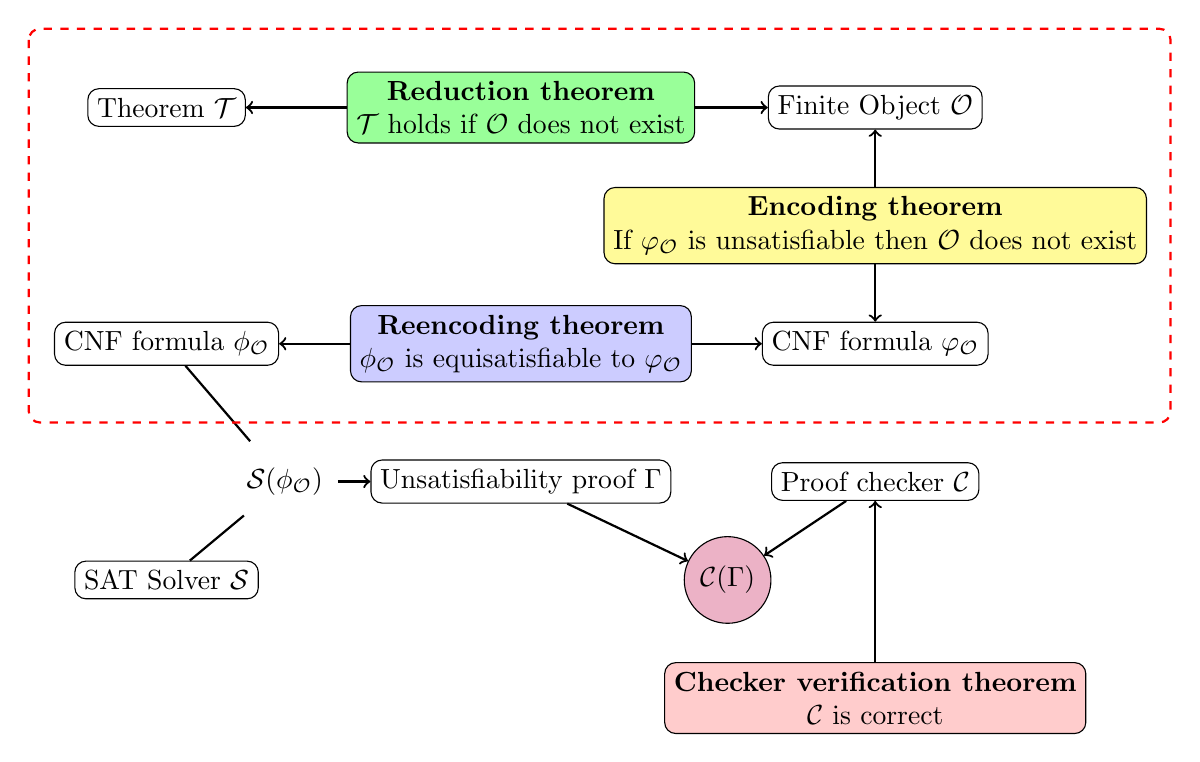
\begin{tikzpicture}
      \node[draw, rounded corners] (theorem) at (0,0) {Theorem $\mathcal{T}$};
      \node[draw, rounded corners] (object) at (9,0) { Finite Object $\mathcal{O}$};
      \node[draw, rounded corners, align=center, fill=green!40!white] (tiffo) at (4.5,0) { \textbf{Reduction theorem}\\$\mathcal{T}$ holds if $\mathcal{O}$ does not exist};
      \draw[->, thick] (tiffo) -- (theorem);
      \draw[->, thick] (tiffo) -- (object);
      \node[draw, rounded corners, align=center] (varphi) at (9, -3) {CNF formula $\varphi_{\mathcal{O}}$};
      \node[draw, rounded corners, align=center, fill=yellow!40!white] (encoding) at (9, -1.5) { \textbf{Encoding theorem}\\If $\varphi_{\mathcal{O}}$ is unsatisfiable then $\mathcal{O}$ does not exist};
      \draw[->, thick] (encoding) -- (object);
      \draw[->, thick] (encoding) -- (varphi);
      \node[draw, rounded corners] (phi) at (0, -3) {CNF formula $\phi_{\mathcal{O}}$};
      \node[draw, rounded corners, align=center, fill=blue!20!white] (equisat) at (4.5, -3) { \textbf{Reencoding theorem}\\$\phi_{\mathcal{O}}$ is equisatisfiable to $\varphi_{\mathcal{O}}$};
      \draw[->, thick] (equisat) -- (phi);
      \draw[->, thick] (equisat) -- (varphi);
      \node[draw, rounded corners] (solver) at (0, -6) {SAT Solver $\mathcal{S}$};
      \node[draw, rounded corners] (unsat-proof) at (4.5, -4.75) {Unsatisfiability proof $\Gamma$};
      \node[circle] (solverphi) at (1.5, -4.75) {$\mathcal{S}(\phi_{\mathcal{O}})$};
      \draw[-, thick] (solver) -- (solverphi);
      \draw[-, thick] (phi) -- (solverphi);
      \draw[->, thick] (solverphi) -- (unsat-proof);
      \node[draw, rounded corners] (checker) at (9, -4.75) {Proof checker $\mathcal{C}$};
      \node[circle, draw, fill=purple!30!white] (checkerphi) at (7.125, -6) {$\mathcal{C}(\Gamma)$};
      \draw[->, thick] (unsat-proof) -- (checkerphi);
      \draw[->, thick] (checker) -- (checkerphi);
      \node[draw, rounded corners, align=center, fill=red!20!white] (checkerCorrectness) at (9, -7.5) { \textbf{Checker verification theorem}\\$\mathcal{C}$ is correct};
  
      \draw[->, thick] (checkerCorrectness) -- (checker);
      \draw[red, dashed, thick, rounded corners] (-1.75,1) -- (-1.75, -4) -- (12.75, -4) -- (12.75, 1) -- cycle;
    \end{tikzpicture}
    \caption{General structure of the verification pipeline for a SAT-based theorem in the \emph{negative case}. The dashed rectangle encloses the main focus of this paper, whereas for the rest of the proof we leverage already existing tools.}\label{fig:proof-structure}
  \end{figure}
The main contribution of this article is to provide the first example of a formally-verified proof of such a theorem in the context of discrete geometry, and the first one overall in Lean, thus addressing different aspects of the question above.
Our proof pipeline involves several components, as illustrated in~\Cref{fig:proof-structure} and described in the rest of the paper.
% \footnote{CC: I'm not sure this characterization is correct. For example, another group of researchers verified in Coq the encoding used in the Pythagorean Triples problem, thus verifying that result. One could say that our contribution is the first \emph{end-to-end} verification, but I don't see how it's inherently distinct from what this other group did with the Pythagorean Triples problem.}

\paragraph{The Empty Hexagon Number.}
In the 1930s, Stein, Erd\H{o}s, and Szekeres mixed geometry and Ramsey theory by studying how many points in the plane in \emph{general position} (i.e., no three points on a common line) are required for a convex $k$-gon to always appear. Let $g(k)$ be the minimum number of points in general position to force a convex $k$-gon.
The celebrated Erd\H{o}s-Szekeres theorem states that $g(k) \leq \binom{2k-4}{k-2} + 1$~\cite{erdosCombinatorialProblemGeometry2009}. Moreover, Erd\H{o}s and Szekeres conjectured that $g(k) = 2^{k-2} + 1$, which has only been proven for $k \leq 6$.

In a similar spirit, Erd\H{o}s defined $h(k)$ as the minimum number of points in general position that is guaranteed to contain a $k$-hole (i.e., a convex $k$-gon without any other point inside).
It is easy to check that $h(3) = 3$ and $h(4) = 5$. In 1978, Harborth established that $h(5) = 10$~\cite{Harborth1978}, and in a surprising turn of events, Horton proved in 1983 that $h(7) = \infty$, meaning one could always avoid $7$-holes~\cite{hortonSetsNoEmpty1983}. 
The only case left open was thus $h(6)$.

The \emph{Empty Hexagon Theorem}, establishing $h(6)$ to be finite, was proven independently by Gerken and Nicolás in 2006, and then refined by Valtr in 2008.
Yet the known range of values for $h(6)$ was quite large, with $29 \leq h(6) \leq 1717$, until Heule and Scheucher used a SAT solver in a recent breakthrough to prove that $h(6) = 30$~\cite{emptyHexagonNumber}, a result we refer to as ``\emph{The Empty Hexagon Number}.''
Now that all the values of $h$ are known, and especially given the extensive computation involved in its proofs, we believe that the final chapter in the story begun by Stein, Erd\H{o}s, and Szekeres is a formal verification of the Empty Hexagon Number.

\paragraph{Related Work.} Despite the crucial role of formal verification in the SAT community (e.g., verified solvers~\cite{oeVersatVerifiedModern2012,skotam_creusat_2022}, proof checking~\cite{lammichEfficientVerifiedSAT2020,tanVerifiedPropagationRedundancy2023}, etc.), the end-to-end formal verification of mathematical proofs obtained through SAT-solving is very recent. To the best of our knowledge, the first and only instance of a formally verified SAT-based mathematical proof before our work corresponds to the Pythagorean Triples Problem, verified in the \textsf{Coq} proof assistant by Cruz-Filipe and Schneider-Kamp~\cite{formalPythagoreanTriples,LPAR-21:Formally_Proving_Boolean_Pythagorean}. In terms of verification of SAT encodings in Lean, the work of Codel, Avigad and Heule pioneered~\cite{Cayden}, while other encoding libraries existed in different frameworks, such as the work of Giljeg\r{a}rd and Wennerbreck in \textsf{CakeML}~\cite{GilAndWennerbeck}, which allowed for verifying SAT-based solutions to different math puzzles (e.g., Sudoku, Kakuro, the \emph{N-queens} problem, etc.).

\paragraph{Outline of the paper.} \Cref{sec:triple-orientations} discusses the basic geometric aspects of the problem, and in particular, \emph{triple orientations} (also known as \emph{signotopes}), a fundamental tool in computational geometry to represent discretely problems involving an a priori continuous space (i.e., $\mathbb{R}^2$), which is the basis of Heule and Scheucher's SAT encoding. Then,~\Cref{sec:symmetry-breaking} deals with two assumptions that are key to break symmetries in the problem and thus make the SAT encoding practically feasible. Namely, that one can assume without loss of generality the following two properties at the same time: (i) points are labeled from left to right without two of them having the same $x$-coordinate, and (ii) the triples $(p_1, p_i, p_j)$ are always oriented counterclockwise for $i < j$. 
\Cref{sec:leansat} presents the \emph{LeanSAT} library, which plays a key role in proving the correctness of encodings. Next,~\Cref{sec:empty-triangle} presents how the previous elements are already enough to formalize a SAT-based proof for the \emph{Empty Triangle Theorem}, a much simpler variant involving only triangles that does not require reencodings. \Cref{sec:empty-hexagon-number} presents the details of the formalization of $h(6) = 30$, the Empty Hexagon Number. We conclude by discussing the next steps towards the formal verification of other Erd\H{o}s-Szekeres-type problems in~\Cref{sec:conclusion}.
